\documentclass[11pt]{article}
\usepackage{fullpage}
\usepackage{graphicx}
\usepackage{float}
\usepackage{amsmath, amsfonts}
\usepackage[utf8]{inputenc}
\usepackage{tabu}

\begin{document}
\begin{figure}[h]
\centering
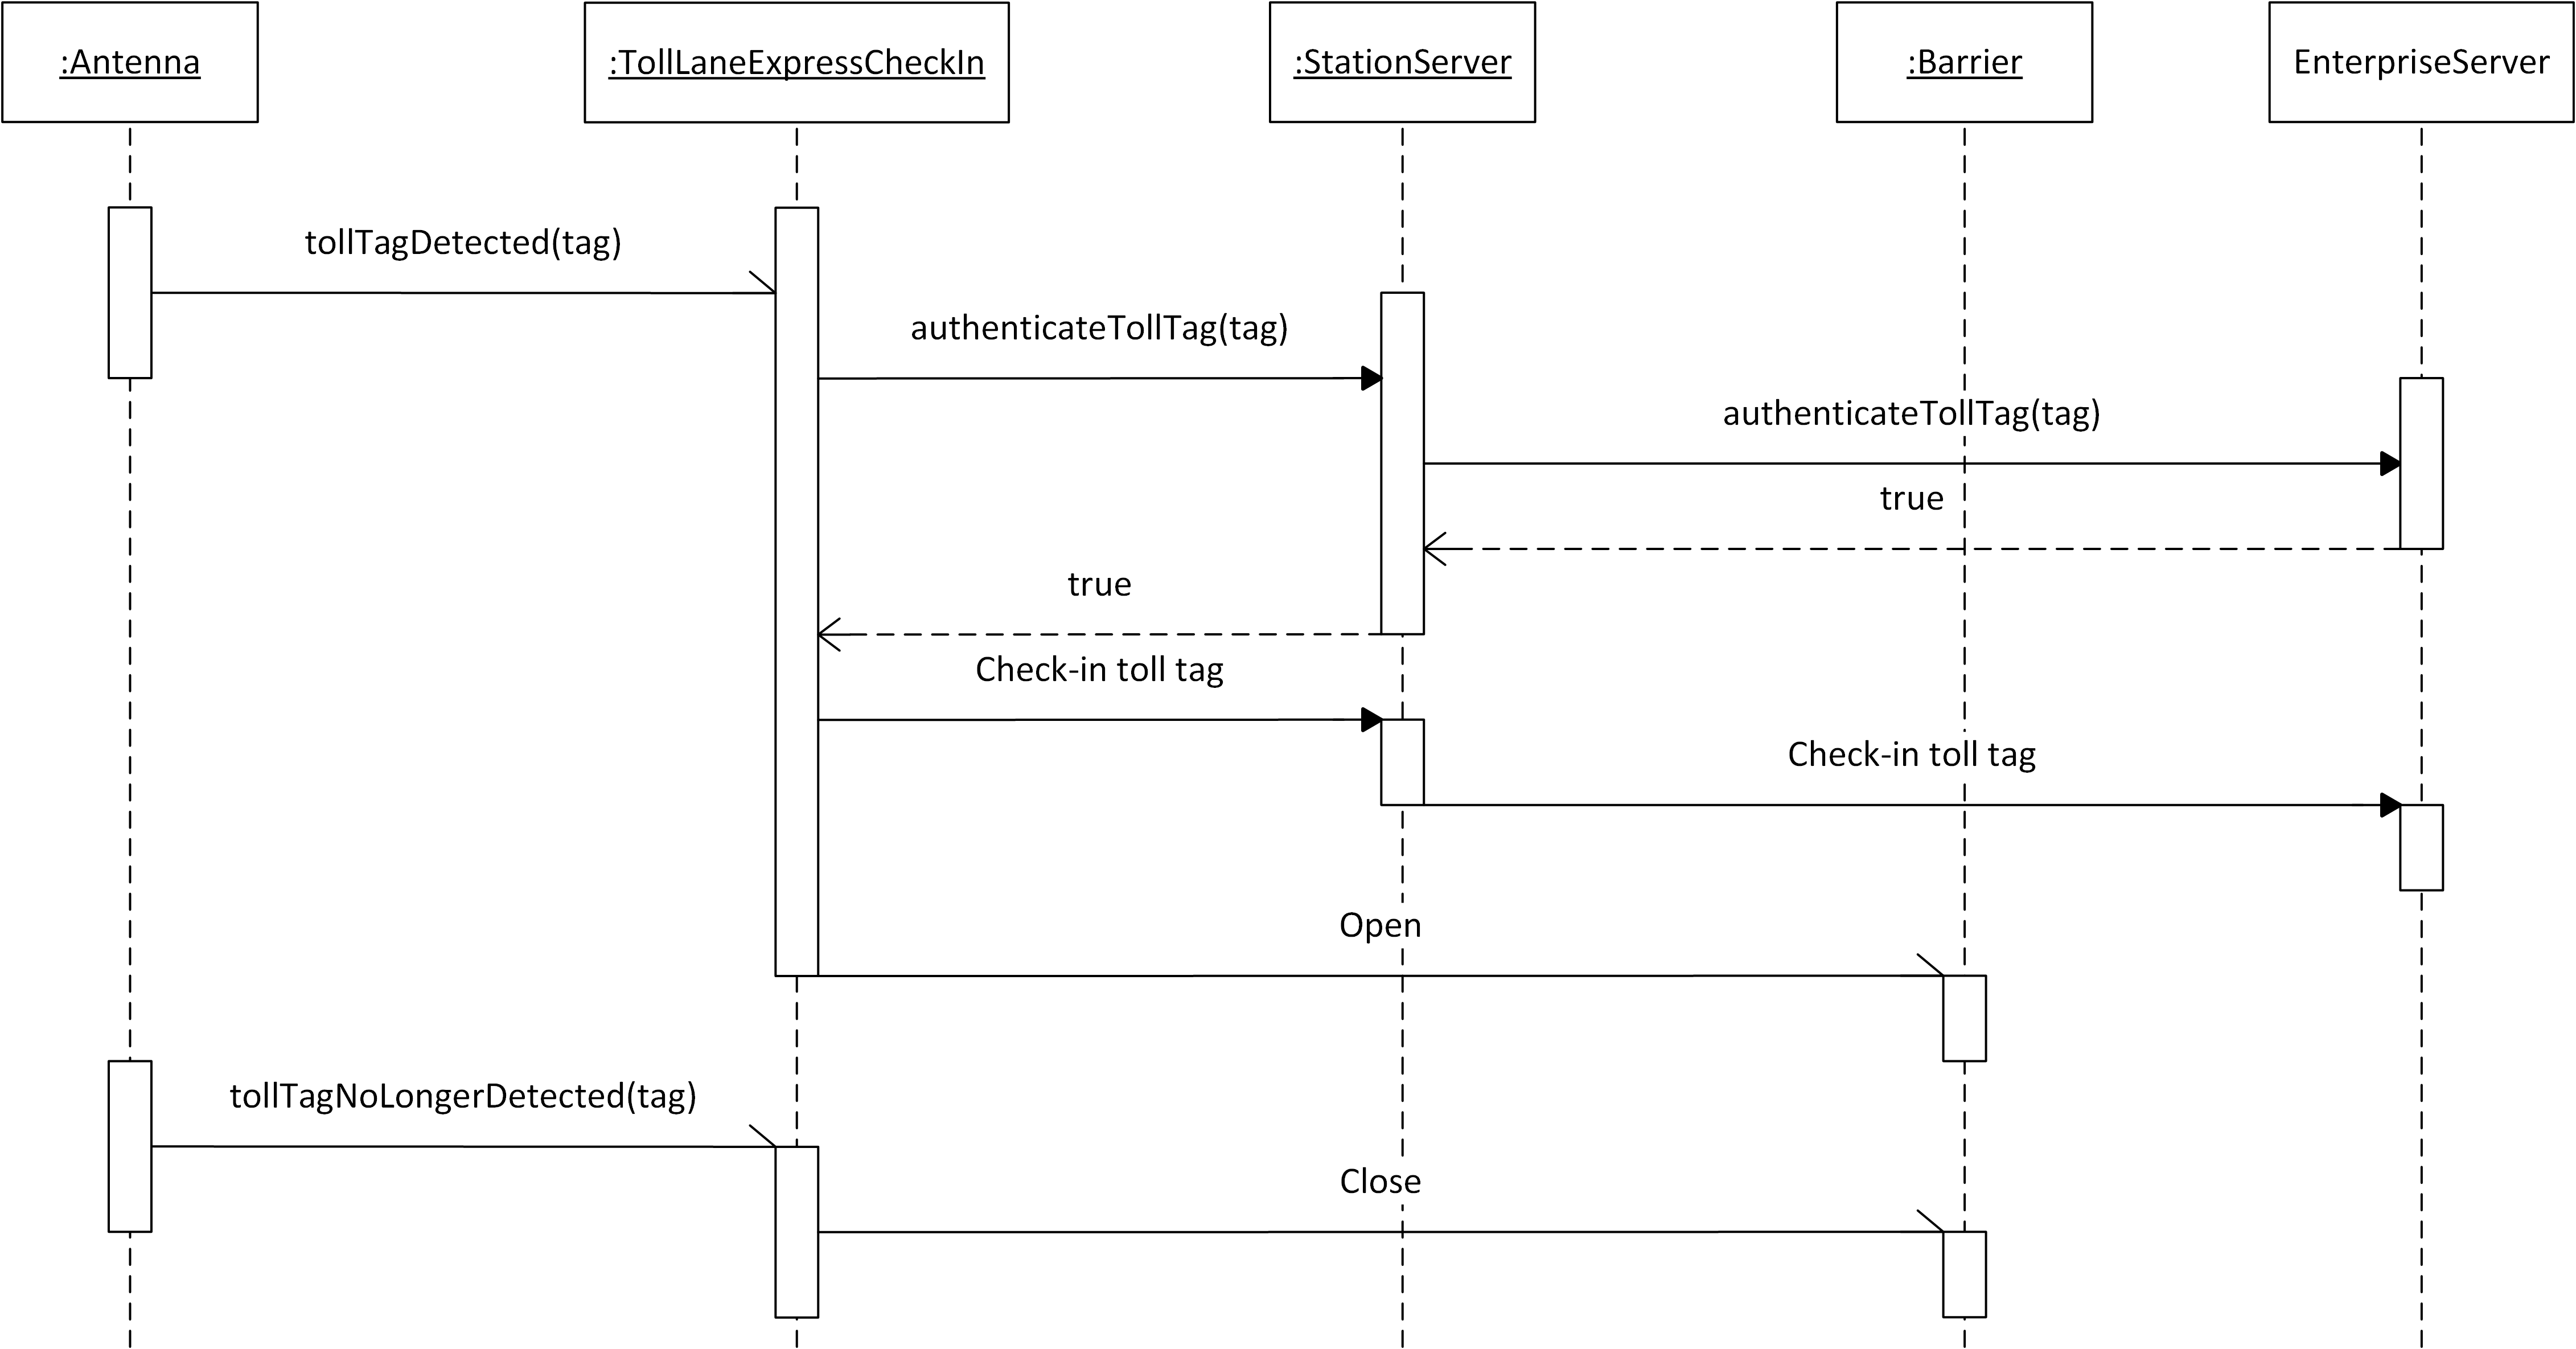
\includegraphics[width=0.7\linewidth]{../report/img/sequence_diagrams/sequence_diagram_toll_tag_check_in.png}
\caption[fig1]{Sequence diagram of single ticket check out}
\label{fig1}
\end{figure}

\begin{enumerate}
\item The customer inserts ticket into the ticket reader.
\begin{enumerate}
\item The ticket reader sends the ticket information in the message readTicket to the 'Toll lane normal check out'-component.
\item The 'Toll lane normal check out'-component tries to validate the ticket using the message validateTicket sent to the station server.
\item The Station server tries to validate the ticket using the message validateTicket sent to the enterprise server.
\item When the ticket is validated the station server stores the ticket data using the method storeCheckOutData.
\item When the validateTicket call returns to the 'Toll lane normal check out'-component, the open message is sent to the barrier.
\end{enumerate}
\item The system opens the  barrier.
\begin{enumerate}
\item The 'Toll lane normal check out'-component calls the method delayForBarrier which gives a delay, based on vehicle type, that allows the customer to pass through.
\end{enumerate}
\item The customer leaves the toll lane.
\begin{enumerate}
\item Once the delay has finished, and the customer hopefully has moved on, the 'Toll lane normal check out'-component sends the close message to the barrier.
\end{enumerate}
\item The system closes the barrier.

\end{enumerate}


\end{document}